% Options for packages loaded elsewhere
\PassOptionsToPackage{unicode}{hyperref}
\PassOptionsToPackage{hyphens}{url}
%
\documentclass[
]{article}
\usepackage{amsmath,amssymb}
\usepackage{iftex}
\ifPDFTeX
  \usepackage[T1]{fontenc}
  \usepackage[utf8]{inputenc}
  \usepackage{textcomp} % provide euro and other symbols
\else % if luatex or xetex
  \usepackage{unicode-math} % this also loads fontspec
  \defaultfontfeatures{Scale=MatchLowercase}
  \defaultfontfeatures[\rmfamily]{Ligatures=TeX,Scale=1}
\fi
\usepackage{lmodern}
\ifPDFTeX\else
  % xetex/luatex font selection
\fi
% Use upquote if available, for straight quotes in verbatim environments
\IfFileExists{upquote.sty}{\usepackage{upquote}}{}
\IfFileExists{microtype.sty}{% use microtype if available
  \usepackage[]{microtype}
  \UseMicrotypeSet[protrusion]{basicmath} % disable protrusion for tt fonts
}{}
\usepackage{xcolor}
\usepackage[margin=1in]{geometry}
\usepackage{longtable,booktabs,array}
\usepackage{calc} % for calculating minipage widths
% Correct order of tables after \paragraph or \subparagraph
\usepackage{etoolbox}
\makeatletter
\patchcmd\longtable{\par}{\if@noskipsec\mbox{}\fi\par}{}{}
\makeatother
% Allow footnotes in longtable head/foot
\IfFileExists{footnotehyper.sty}{\usepackage{footnotehyper}}{\usepackage{footnote}}
\makesavenoteenv{longtable}
\usepackage{graphicx}
\makeatletter
\def\maxwidth{\ifdim\Gin@nat@width>\linewidth\linewidth\else\Gin@nat@width\fi}
\def\maxheight{\ifdim\Gin@nat@height>\textheight\textheight\else\Gin@nat@height\fi}
\makeatother
% Scale images if necessary, so that they will not overflow the page
% margins by default, and it is still possible to overwrite the defaults
% using explicit options in \includegraphics[width, height, ...]{}
\setkeys{Gin}{width=\maxwidth,height=\maxheight,keepaspectratio}
% Set default figure placement to htbp
\makeatletter
\def\fps@figure{htbp}
\makeatother
\setlength{\emergencystretch}{3em} % prevent overfull lines
\providecommand{\tightlist}{%
  \setlength{\itemsep}{0pt}\setlength{\parskip}{0pt}}
\setcounter{secnumdepth}{-\maxdimen} % remove section numbering
% definitions for citeproc citations
\NewDocumentCommand\citeproctext{}{}
\NewDocumentCommand\citeproc{mm}{%
  \begingroup\def\citeproctext{#2}\cite{#1}\endgroup}
\makeatletter
 % allow citations to break across lines
 \let\@cite@ofmt\@firstofone
 % avoid brackets around text for \cite:
 \def\@biblabel#1{}
 \def\@cite#1#2{{#1\if@tempswa , #2\fi}}
\makeatother
\newlength{\cslhangindent}
\setlength{\cslhangindent}{1.5em}
\newlength{\csllabelwidth}
\setlength{\csllabelwidth}{3em}
\newenvironment{CSLReferences}[2] % #1 hanging-indent, #2 entry-spacing
 {\begin{list}{}{%
  \setlength{\itemindent}{0pt}
  \setlength{\leftmargin}{0pt}
  \setlength{\parsep}{0pt}
  % turn on hanging indent if param 1 is 1
  \ifodd #1
   \setlength{\leftmargin}{\cslhangindent}
   \setlength{\itemindent}{-1\cslhangindent}
  \fi
  % set entry spacing
  \setlength{\itemsep}{#2\baselineskip}}}
 {\end{list}}
\usepackage{calc}
\newcommand{\CSLBlock}[1]{\hfill\break\parbox[t]{\linewidth}{\strut\ignorespaces#1\strut}}
\newcommand{\CSLLeftMargin}[1]{\parbox[t]{\csllabelwidth}{\strut#1\strut}}
\newcommand{\CSLRightInline}[1]{\parbox[t]{\linewidth - \csllabelwidth}{\strut#1\strut}}
\newcommand{\CSLIndent}[1]{\hspace{\cslhangindent}#1}
\usepackage{setspace}
\usepackage{caption}
\ifLuaTeX
  \usepackage{selnolig}  % disable illegal ligatures
\fi
\usepackage{bookmark}
\IfFileExists{xurl.sty}{\usepackage{xurl}}{} % add URL line breaks if available
\urlstyle{same}
\hypersetup{
  pdftitle={Inferring Treatment Resistance Actively: Modifying Partially Observable Markov Decision Processes for Adaptive Therapy},
  pdfauthor={Emil Frej Brunbjerg, Social and Cultural Dynamics, BSc. Cognitive Science, Aarhus University},
  hidelinks,
  pdfcreator={LaTeX via pandoc}}

\title{Inferring Treatment Resistance Actively: Modifying Partially
Observable Markov Decision Processes for Adaptive Therapy}
\author{Emil Frej Brunbjerg, \n Social and Cultural Dynamics, BSc.
Cognitive Science, Aarhus University}
\date{2024-05-28}

\begin{document}
\maketitle
\begin{abstract}
\doublespacing Cancer remains a leading cause of death globally, with
drug resistance accounting for approximately 90\% of cancer fatalities.
\emph{Adaptive Therapy} (AT) which leverages intra-tumoral evolutionary
dynamics to control rather than eradicate cancer, is a promosing
alternative to standard care. This paper investigates if the
\emph{Active Inference} (AI) \emph{Partially Observable Markov Decision
Process} (POMDP) scheme to model and control cancer dynamics in a
simulated enviroment inspired by a recent pilot clinical trial that
implements AT for metastastic-Castration Resistant Prostate Cancer. The
problem of inferring resistance dynamics based on signals of tumor
burden motivated the use of AI, but also necesistaed modifying how
transition dynamics are specified and evaluated in the POMPD scheme.
Intial simulation results suggest that the modification allowed POMDPs
to infer changes to resistance dynamics in real-time through observing
changes in tumor burden resulting from applying treatment. The modified
POMPDs were also tested against a range-bounded treatment strategy
inspired by the pilot trial, and found to outperform the range-bounded
strategy, particularly under conditions of aggresive tumor growth.
Beyond the intially promising simulation results, POMDPs were also found
to meet several criteria that have recently been identified as crucial
for modelling work in AT. Consequently, this paper argues that the AI
paradigm shows promise for improving real-time prediction of treatment
responses, particularily when AI is applied through POMDPs.
Additionally, the paper indentifies key developments needed before the
POMPD scheme can be applied in clinical settings, and suggests that
developing a rigorous benchmarking suite would propel modelling efforts
in AT. \clearpage
\end{abstract}

{
\setcounter{tocdepth}{3}
\tableofcontents
}
\setstretch{2}

\captionsetup[figure]{font=scriptsize}

\pagebreak

\section{Introduction}\label{introduction}

\subsection{A Primer on Adaptive
Therapy}\label{a-primer-on-adaptive-therapy}

Worldwide, cancer is the cause of 1 out of 6 deaths. An estimated 90\%
of these cancer deaths are due to the development of drug resistance
(Bukowski, Kciuk, and Kontek 2020). While initial cancer treatment
usually shows a positive response in tumor burden, drug resistance
develops over time. To highlight the inefficiency of traditional
approaches, (Staňková et al. 2019) models cancer treatment as a
game-theoretic contest between a physician and a tumor. In this model,
the physician's move in each round is to apply a certain treatment to
which the cancer adapts. While the game is assymetrical---one player is
the leader (the physician) and another player is a follower (the
tumor)---the asymmetry is rarely exploited in oncology wards. Instead of
using the advantage to steer the evolutionary pressures placed on
tumors, tumors can adapt not only to the current round of the game but
also to future rounds under standard care. Thus, the advantage of
leading the game is lost. The authors analogize the current practice to
a game of rock-paper-scissors:

\begin{quote}
\emph{'' in which almost all cells within the cancer play, for example,
``paper.'' It is clearly advantageous for the treating physician to play
``scissors.'' Yet, if the physician only plays ``scissors,'' the cancer
cells can evolve to the unbeatable resistance strategy of ``rock.''``}
(Staňková et al. 2019).
\end{quote}

To exploit this asymmetry \emph{Adaptive Therapy} (AT) controls
intra-tumoral evolutionary dynamics by leveraging that cancer cells
likely incur fitness costs when evolving mechanisms of drug resistance
(Gatenby et al. 2009). If resistant and non-resistant cells are
competing for space and resources, drug-sensitive cells should, over
time, out-compete resistant cells. AT thereby utilizes Darwinian
competition to make cancer suppress itself, a strategy that potentially
could reduce cancer to chronic and but controllable disease.

\begin{figure}
\centering
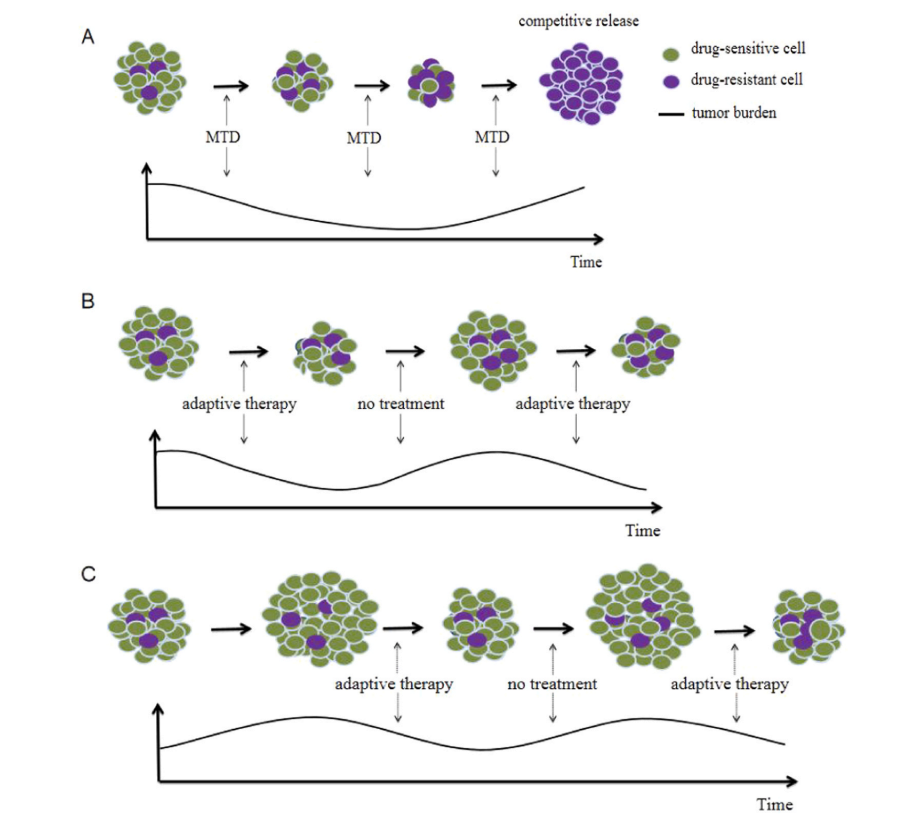
\includegraphics[width=3.125in,height=\textheight]{images/Screenshot 2024-05-20 at 08.15.19.png}
\caption{From Zhang et al.~2023. Panel A shows a typical ``Maximal
Tolerable Dose'' treatment protocol. While the initial response in tumor
burden is promising, a competitive release of resistant cells ensures.
Panel B shows an AT approach with a small tumor burden. Panel C shows AT
with a high tumor burden, which has been theorized to further increase
the suppression of resistance cells.}
\end{figure}

Initial results from an ongoing pilot clinical trial applying AT in a
group of \emph{metastatic castrate-resistant prostate cancer} (mCRPC)
patients are promising, showing both lower cumulative dosages and longer
survival times compared to a similar group of patients receiving
standard care. The trial utilizes a range-bounded heuristic to make
treatment decisions: if the blood marker \emph{Prostate-specific
Antigen} (PSA), a proxy for tumor burden, increases back to pre-trial
levels, Abiraterone treatment is applied until PSA drops to 50\% of
pre-trial levels (Zhang et al. 2017).

\subsection{POMPDs}\label{pompds}

\emph{Partially Observable Markov Decision Processes} (POMDPs) is a
class of controller models that model a Markov process ---an environment
that moves through discrete time steps and states, each step of the
system only depends on states of the prior step. Partial observability
refers to the fact that these models don't directly observe the actual
environment but instead observe signals emitted by the environment
(Åström 1969). This allows POMPDs to differentiate an observed signal
from what it ``believes'' about the actual configuration of states and
additionally to use a single reward function to trade-off uncertainty
for reaching a certain goal state (Kaelbling, Littman, and Cassandra
1998).

\subsection{Solving POMPDs with Active
Inference}\label{solving-pompds-with-active-inference}

While POMDPs are typically difficult to solve analytically, various
approximation exist. One approximation scheme is born out of the
neuroscience paradigm \emph{Active Inference} (AI) where POMPDs are
typically used to model an agent's decision-making. AI POMPDs has been
used to model psychopathology (Da Costa et al. 2020) but also applied to
control scenarios such as the mountain car problem (Friston, Daunizeau,
and Kiebel 2009) and, albeit augmented with deep learning, robotics
control (Çatal et al. 2020). The approximation finds a solution by
minimizing two objective functions:

\begin{itemize}
\item
  \emph{Variational Free Energy} (VFE). A measure of fit between a
  generative model and sensory input.
\item
  \emph{Expected Free Energy} (EFE). A score of how well a course of
  action is expected to bring about a set of preferences penalized for
  expected uncertainty.
\end{itemize}

AI implementations of the POMDP scheme have been implemented in MATLAB
and recently in Python with the Python package \emph{pymdp} Heins et al.
(2022a). AI POMDPs are technically the a joint probability:

\[
p(o,s,u;\phi)
\]

where \(o\) are observations, \(s\) are hidden states to be inferred,
\(u\) are actions that an agent can take to influence the environment,
and \(\phi\) are the hyperparameters of the model, such as \(\alpha\)
normally used as `inverse temperature' i.e.~how strongly beliefs
determines action selection. By conditioning on certain observations,
the POMDP is solvable for Bayes-optimal posterior beliefs at a given
time point. This yields a set of posterior beliefs about the current
state of each \emph{state factor -} the types of possible states in the
environment. A posterior probability distributions over what
\emph{policies}, possible courses of actions are most likely to achieve
specified preferences while keeping expected uncertainty as low as
possible. As an example, a POMDP could model the joint probability of
observing a noisy signal of a particular tumor burden in a patient, an
actual underlying tumor burden, and the course of action that is most
likely to bring the tumor burden down. By modeling, actions, states, and
observations as discrete events, the joint probability is can factorized
into multiple categorical probability distributions. These describe
likelihood mappings between signals and specific states of the
environment, transition probabilities, and a desired probability of
making certain observations (see appendix A for an in-depth description
of how an agents generative model is specified by factorizing the joint
probability). Solving (Smith, Friston, and Whyte 2022). \footnote{The
  Python package pymdp (Heins et al. 2022b) has numerous tutorial
  notebooks for implementing POMPDs in Python. Smith, Friston, and Whyte
  (2022) describes the process of constructing POMPDs for different
  scenarios in detail, albeit in MATLAB, and Da Costa et al. (2020)
  provides an in-depth mathematical account of POMPDs in Active
  inference.}

\subsection{Aim of this Paper}\label{aim-of-this-paper}

The treatment decisions used in the pilot trial reported by Zhang et al.
(2017) were based on a well-informed heuristic about how resistance
dynamics would develop as a consequence of careful timing of applying
and withdrawing Abiraterone treatment. However, the actual resistance
dynamics of each patient weren't explicitly modeled in real-time, and
thus not used in treatment decisions. This paper primarily investigates
whether the AI implementation of POMDPs can model and control degree of
treatment resistance of individual cancer patients in real-time ---
hoping that this strategy eventually can be applied in a clinical
setting.

\section{Analysis}\label{analysis}

\subsection{Simulated environment}\label{simulated-environment}

To investigate the appropriateness of the AI implementation of the POMDP
scheme, multiple simulations of a clinical setting inspired by the pilot
clinical trial were run. To comply with the canonical AI POMPD scheme
discrete states and and time steps were used. Each simulation run
simulated maximally of 200 time-steps. At each time-step, an agent had
to keep a virtual cancer patient alive by deciding whether to apply a
treatment based on a signal of the tumor burden. The signal could be
observed at each time point, and treatment decisions were made by
solving a slightly modified AI POMPD. The features of the environment
were inspired by the use of PSA testing and Abiraterone treatment in the
pilot trial (Zhang et al. 2017). In the simulations, the patient's
\emph{tumor state factor} determined whether they survived to the next
time-step. If the tumor state factor reached the maximal state of six
possible states, the virtual patient ``died'' and the simulation ended.
The tumor state factor was always set to the lowest at the beginning of
each simulation run and could increase at a fixed risk at each time
step.

Whether a round of treatment successfully reduced the tumor state
depended on an underlying \emph{resistance state factor}. This also
began at state 0 out of 5. For each round of treatment application, the
resistance state had a fixed risk of increasing. The only remedy to the
increasing resistance states, beyond favorable bouts of stochasticity,
was to withdraw treatment which would allow the resistance state factor
to lower. Inspired by the work of (Hansen and Read 2020), the patient
being higher tumor states increased the chance of lowering resistance.

\subsection{Modifications to the POMDP
Scheme}\label{modifications-to-the-pomdp-scheme}

Typically when constructing AI POMDPs, different state factors (i.e
types of states) such as the resistance factor and tumor factors are not
modeled to affect each other directly. Instead, the interactions
resulting from of particular specific states across state types are
modeled as leading to different observations. This means that
interactions between types of states would be coded in the likelihood
distribution.

This setup was deemed incompatible with the environment that the agents
had to model since it wouldn't let agents infer how changes in
resistance state factor should influence the expected transition
probabilities of the tumor state factor. Therefore, custom changes were
made to pymdp to allow POMPDs to infer ``occluded'' state factors -
state factors don't produce signals themselves (e.g.~the resistance
state). The state of the occluded state factor need to be inferred,
through its effects on downstream state factors that generate signals
(e.g.~the tumor state).

Specifically, modifications were made to the structure of the agents
beliefs about the environment's transition probabilities Usually,
three-dimensional \emph{tensors} describe expected transition
probabilities within a state factor. This means a tensor for a type of
state typically holds one dimension for the current state, one dimension
for the next state, and a third dimension for every allowed action. Each
cell of the tensor then contains the probability of transitioning from
one state to another state conditional on a certain action. Another
dimension was added to relevant tensors. This dimension corresponded to
another state factor. Concretely, this means that the tensor for tumor
transition probabilities had a fourth dimension corresponding to the
possible resistance states. The expected transition probabilities could
then be estimated by matrix multiplying the tumor transition tensor with
a vector containing expected probabilities of each resistance state at a
given time point. One can imagine that instead of having only one tensor
for the transition probabilities between tumor states, multiple tensors
of tumor transition probabilities were specified, where each tensor
corresponded to a specific resistance level. This modification to the
generative model necessitated taking an average of across these tensors
weighted by the posterior probabilities for each resistance state at
given time point. This amounts to calculating the expected transition
probabilities between tumor states conditional on a set of beliefs about
the resistance states. This modification strategy was repeated for the
resistance level since decreases in the resistance state depended on the
tumor state. It should be noted that this modification means that the
order in which beliefs about states are evaluated must be specified.
While these changes rendered much of the functionality of pymdp
immediately unusable, the modification strategy should be able to model
arbitrarily complex dependencies between states.

\subsection{Exploratory Simulation}\label{exploratory-simulation}

An exploratory simulation was conducted, where for each run an agent
instantiated as a modified POMPD controlled whether to treat and test.
Its received the following signals:

\begin{itemize}
\item
  A noiseless signal of whether the patient was alive.
\item
  A noiseless signal of whether it was applying tests.
\item
  A noiseless signal of whether it was applying treatment
\item
  A noised signal of the tumor state and it was only recieved if tests
  were being applied.
\end{itemize}

The agent's prior preferences were skewed heavily against observing a
dead patient, somewhat against treating, and slightly against testing.
This was done to simulate the cost to both treating and testing. This
means that the agent had to balance the cost of its actions while
considering the potential information gain of each choice. The costs of
treating and testing were introduced to investigate whether the POMPD
scheme could potentially be used to strike a balance between drug
toxicity, and tumor burden while optimizing real-time data collection as
desired by key researches in AT (West et al. 2020). The model was
further handicapped by noising the tumor signal. This means that the
resistance state, which had to be inferred through the tumor signal, was
doubly obfuscated.

However, the agent's generative model did perfectly map the expected
noise in the tumor signal, and its initial expected transition
probabilities were identical to the actual transition probabilities of
the environment. Additionally, the agent was given uniform priors over
initial states, meaning it had no knowledge of the configuration of
states at the beginning of each run. The same set of predetermined
policies that considered the next 6 time-steps were evaluated at each
step. This limited set of policies was done to ease computation by
limiting the search space of possible actions. The set of policies
consisted of two blocks of either testing or treating for three
time-steps in a row for permuted each possible sequence of applying
testing or not for the time horizon of the policies.

\subsubsection{Inferring the Resistance
State}\label{inferring-the-resistance-state}

In the following example of an exploratory simulation run, the agent
managed to keep the patient alive for 68 time-steps and chose to test on
55 of these (see Fig. 2).

\begin{figure}

{\centering 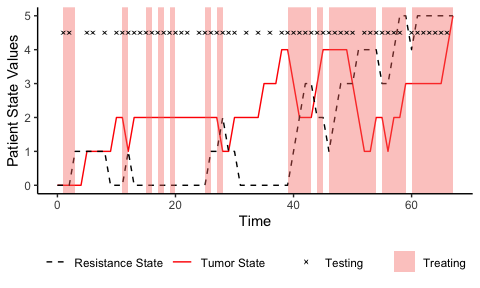
\includegraphics{SocultPaperV7_files/figure-latex/sim run-1} 

}

\caption{A simulation run for exploratory purposes. The simulation ended before time-step 200 since the simulated patient "died" when the tumor state factor reached the state 5.}\label{fig:sim run}
\end{figure}

The agent appears to be somewhat sensibly applying treatment, but it
doesn't apply the treatment at a pivotal period approximately between
steps 30 and 39. Interestingly, the agent decides to apply treatment at
the first timestep, despite the tumor state and resistance state being
at their lowest possible values. Considering that the generative model
had uniform priors over both resistance state and tumor states, this
behavior is appropriate from the perspective of the agent, since
treating and testing would immediately provide information about both
states. The model further seemed to prefer testing when treatment is
being applied. This suggests that it found testing to be more worthwhile
while also treating. Given that by combining treatment and testing, the
agent can learn about both the resistance and tumor state factors, all
else being equal, the expected information gain should therefore be
increased by this behavior. A plot of the model's beliefs about the
resistance state at each time-point (see Fig. 3) shows that its beliefs
about the resistance state generally follow the development of the
actual resistance state despite the lack of direct signal.

\begin{figure}

{\centering 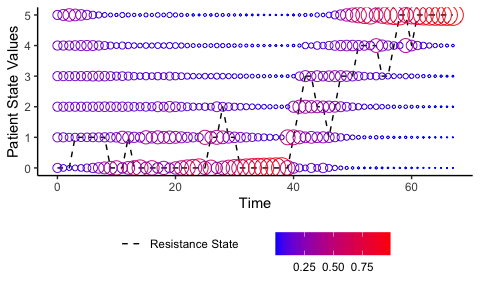
\includegraphics{SocultPaperV7_files/figure-latex/res beliefs-1} 

}

\caption{Agents beliefs about the patient's resistance  state at every timepoint. Size and color of circles indicate the probability that the agent assigns to each value of the state at a given time-step.}\label{fig:res beliefs}
\end{figure}

In summary, the modification to POMPD structure appears to have allowed
the agent to infer the occluded resistance states in real-time. While
the results are initially promising, the particular agent did make
questionable choices regarding the timing of treatment. It's
decision-making is dissected in-depth in Appendix C.

\subsection{Performance of POMPDs against a Range-Bounded
Strategy}\label{performance-of-pompds-against-a-range-bounded-strategy}

Several agents instantiated as modified POMPDs were tested against a
range-bounded strategy. This was done to benchmark the performance of
POMPDs against a strategy inspired by the treatment protocol used in the
pilot clinical trial (Zhang et al. 2017). The generative models used
were simplified for ease of computation --- they only observed a
noiseless signal of the tumor state and whether treatment was being
applied at every time-step. They were also only given prior preferences
for observations of tumor states. The preferences were uniform over all
survivable observations of survivable tumor burdens, and the probability
of the observing the maximal burden was set to 0. The following three
agents were tested:

\begin{itemize}
\tightlist
\item
  A short policy horizon POMPD that could consider a block of treating
  or not treating for the next three steps.
\item
  A medium policy horizon POMPD that could consider two blocks of
  treating or not treating for three steps, yielding a total horizon of
  6 timesteps.
\item
  A long policy horizon POMPD that could consider four blocks of
  treating or not treating for three steps, resulting in a total horizon
  of 12 steps.
\end{itemize}

The agents were benchmarked on four different tumor growth rates, to
investigate how a cancer's aggresiveness would affect the agent's
ability to keep patients alive. The tested tumor growth rates were 0.1,
0.3, 0.5, and 0.7 probability of an increase in tumor state at each
timestep. For each setting, 100 simulation were run. For each run, the
environment was predetermined by generating 200 outcome variables for
each combination of tumor state, resistance state, and treatment state
to ensure comparability between the tested agents and the RB strategy at
the level of each run.

\begin{figure}

{\centering 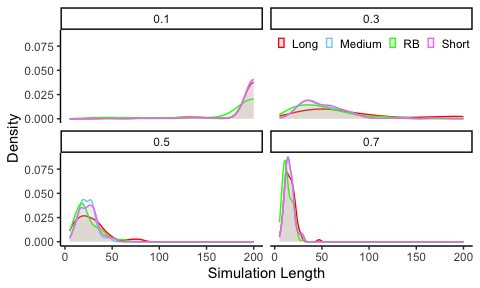
\includegraphics{SocultPaperV7_files/figure-latex/sim lengths-1} 

}

\caption{Simulated observed patient survival times for each POMPD agent and the range-bounded strategy.}\label{fig:sim lengths}
\end{figure}

At the lowest tumor growth rate, nearly all the runs reached the maximal
length (see Fig. 4). On the other runs, the long horizon model also
appears to be slightly outperforming the others. Contrasts as the
percentage difference in survival from switching from the baseline
RB-strategy to the long horizon POMPD are computed for each run (see Fig
5.).

\begin{figure}

{\centering 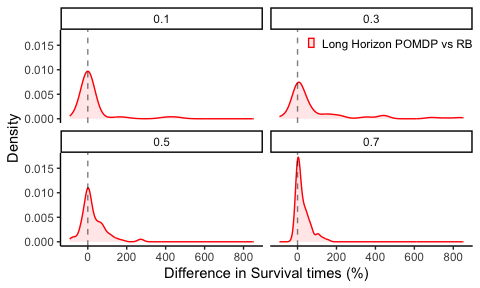
\includegraphics{SocultPaperV7_files/figure-latex/constrasts-1} 

}

\caption{Change in percent of between the range-bound approach and the longest horizon POMPD for different tumor growth rates.}\label{fig:constrasts}
\end{figure}

In the 100 runs with a 0.1 risk of tumor growth, the long-horizon POMPD
seems to perform similarly to the RB strategy. However, as the tumor
growth risk increases, the POMPD agent increasingly shows large
percentage improvements compared to the RB strategy. Potentially a
consequence of a greater need for proactive action when tumor dynamics
accelerate, which in turn could favor models that explicitly model how
treatment will effect future resistance dynamics.

\section{Discussion}\label{discussion}

\subsection{Findings}\label{findings}

This project tested a modification to how POMDPs are typically
implemented in AI to investigate whether POMDPs could infer and control
state factors that don't emit signals, but instead influence other state
factors. This was accomplished. In a simulated environment designed to
mimic the dynamics of AT, the modification allowed agents instantiated
as POMDPs to model an underlying resistance state that controlled the
efficacy of cancer treatment, despite the underlying state not producing
observable signals itself.

Modified POMPDs were further tested against a range-bounded treatment
strategy inspired by a pilot clinical trial using AT, and were found to
outperform the range-bounded strategy substantially. The gap in
performance was largest in simulations of aggressive tumor growth rates
and for agents with an ability to consider longer future courses of
action. These results in concert with a recent review of needed
developments in AT models (West et al. 2023) underscore the potential of
drawing inspiration in the AI paradigm for real-time planning of
treatment and testing decisions. Perhaps the modified POMDP could be a
useful model architecture that,with refinement, could come to improve
real-time patient-specific therapy treatment decisions.

This paper implemented a POMPD capable of combining multiple actions,
i.e.~treating and testing. Only computation and our ability to specify
likelihood and transition probabilities prohibit constructing more
complex generative models. Potentially opening the door for combining
multi-drug therapies with multiple types of testing and increasingly
detailed models of real-time tumor biology --- all of which are
desiderata reported by West et al. (2023).

But to avoid having to figure out how quarks and leptons might interact
to produce a cancer cell, we will have to limit our desire for higher
causal resolution at some point. While simulating finer-grained
mechanisms of tumor biology likely will benefit clinical adaptions of
AT, abstracting away physical mechanisms as random fluctuations inherent
to the modeled environment will eventually be necessary. Models for
real-time treatment decisions will therefore have to need the capacity
to model the uncertainty of the environment and account for it in
decision-making .

Another quality of the AI paradigm is its ability to quantitatively
incorporate expected utility and uncertainty in decision-making. In
doing so, these models blur the line between testing and treating. For
example, a model could correctly believe that two patients have exactly
the same tumor burden but suggest treatment for one patient and not the
other. This is a feature, not a bug. If the model is certain in its
beliefs about one patient's resistance dynamics, the expected gain in
information from treating will be small. Yet if the model is uncertain
about the resistance dynamics of the other patient, it might be
worthwhile to apply treatment simply for the information gain.
Curiously, this could result in two patients with exactly the same tumor
burden, but only one of them should receive treatment. Factoring in
measures of uncertainty drastically alters how to optimally collect
real-time data patient data. It would allow for a carefull and
quantitative reasoning of when to use treatment responses to investigate
resistance dynamics. Treatment responses were implicitly used as an
information gathering tool in the pilot trial, Zhang et al. (2017)
report only including patients who showed a substantial drop in PSA
after an initial round of treating, but models in inspired in AI could
carefully and quantitatively balance information gathering against other
objective measures such as drug toxicity, patient well-being, emergence
of resistance or financial costs.

\subsection{Suggestions for Future
Research}\label{suggestions-for-future-research}

While the results are initially promising, the simple nature of the
simulated clinical setting prohibits drawing any strong conclusions
about the promise of using AI POMPDs in a clinical setting.

To further investigate whether POMDPs could viably be applied in a
clinical setting, multiple problems will need to be solved. For example,
in the present study, the environment featured only discrete values.
Since biomarkers and dosage intensities will likely take continuous
values, some combination of binning continuous values to discrete values
or adapting the model structure to work with continuous data is
necessary. In the face of similar constraints, deep learning has been
used to construct likelihood mappings and transition probabilities in
POMDPs (Çatal et al. 2020). Finding better methods for searching the
policy spaces will likely also be pivotal --- Da Costa et al. (2020)
suggest how the space of possible actions could be pruned to decrease
search times.

Another key issue is determining a how to inform likelihood and
transition probabilities in a fashion that is compatible with a clinical
setting. The present study used the actual transition probabilities of
the simulated environment and, depending on the simulation run,
noiseless likelihood mappings. Possibly, simulations of cancer dynamics,
such as those by Zhang et al. (2017), could be used to inform transition
probabilities, and a clinical model could potentially readjust to
patient data. The AI implementation of POMDPs has developed literature
on online learning of the categorical probability distributions needed
to accurately represent the environment. Even potential information
gains from learning transition and likelihood probabilities can be
factored in to decision-making Da Costa et al. (2020).

In the present paper, the ranges of the baseline range-bounded strategy
were selected arbitrarily --- the chosen range produced managed to
control tumor states for a substantial amount of time. A systematic
method for comparing models could ease comparison of models. Choice of
modeling framework, building a benchmarking could help propel modeling
work in AT. The work of West et al. (2023) could potentially be
translated to a set of simulation environments used for benchmarking.
Wrapping existing simulations into environments that can easily
facilitate actions and observations with simulated agents could be done
by using an API like the one used in Gymnasium (formerly OpenAI Gym)
(Towers et al. 2024). This would hopefully minimize friction for
non-oncology researchers wishing to contribute to the field by allowing
them to prioritize improving model performance over spending excessive
time deciphering how to construct useful metrics themselves.

POMPDs could also be ``reverse-engineered'' from more complex models,
which could more easily be trained if a benchmarking suite existed. For
example, if a black-box model, like a neural network, can be shown to
successfully control treatments, fitting a POMPD to its behavior would
probably be a fairly straight-forward endeavor since AI POMPDs often
have been used in computational psychiatry to model human
decision-making. The same techniques could potentially allow us to
translate otherwise non-transparent models into the structure of a
POMPD, thus combining the performance of the black-box model with the
transparency of the POMPD scheme.

\section{References}\label{references}

\phantomsection\label{refs}
\begin{CSLReferences}{1}{0}
\bibitem[\citeproctext]{ref-uxe5struxf6m1969}
Åström, K. J. 1969. {``Optimal Control of Markov Processes with
Incomplete State-Information II. The Convexity of the Lossfunction.''}
\emph{Journal of Mathematical Analysis and Applications} 26 (2): 403--6.
\url{https://doi.org/10.1016/0022-247X(69)90163-2}.

\bibitem[\citeproctext]{ref-bukowski2020}
Bukowski, Karol, Mateusz Kciuk, and Renata Kontek. 2020. {``Mechanisms
of Multidrug Resistance in Cancer Chemotherapy.''} \emph{International
Journal of Molecular Sciences} 21 (9): 3233.
\url{https://doi.org/10.3390/ijms21093233}.

\bibitem[\citeproctext]{ref-uxe7atal2020}
Çatal, Ozan, Samuel Wauthier, Cedric De Boom, Tim Verbelen, and Bart
Dhoedt. 2020. {``Learning Generative State Space Models for Active
Inference.''} \emph{Frontiers in Computational Neuroscience} 14
(November). \url{https://doi.org/10.3389/fncom.2020.574372}.

\bibitem[\citeproctext]{ref-dacosta2020}
Da Costa, Lancelot, Thomas Parr, Noor Sajid, Sebastijan Veselic,
Victorita Neacsu, and Karl Friston. 2020. {``Active Inference on
Discrete State-Spaces: A Synthesis.''} \emph{Journal of Mathematical
Psychology} 99 (December): 102447.
\url{https://doi.org/10.1016/j.jmp.2020.102447}.

\bibitem[\citeproctext]{ref-friston2009}
Friston, Karl J., Jean Daunizeau, and Stefan J. Kiebel. 2009.
{``Reinforcement Learning or Active Inference?''} \emph{PLoS ONE} 4 (7):
e6421. \url{https://doi.org/10.1371/journal.pone.0006421}.

\bibitem[\citeproctext]{ref-gatenby2009}
Gatenby, Robert A., Ariosto S. Silva, Robert J. Gillies, and B. Roy
Frieden. 2009. {``Adaptive Therapy.''} \emph{Cancer Research} 69 (11):
4894--4903. \url{https://doi.org/10.1158/0008-5472.CAN-08-3658}.

\bibitem[\citeproctext]{ref-hansen2020}
Hansen, Elsa, and Andrew F. Read. 2020. {``Modifying Adaptive Therapy to
Enhance Competitive Suppression.''} \emph{Cancers} 12 (12): 3556.
\url{https://doi.org/10.3390/cancers12123556}.

\bibitem[\citeproctext]{ref-heins2022a}
Heins, Conor, Beren Millidge, Daphne Demekas, Brennan Klein, Karl
Friston, Iain D. Couzin, and Alexander Tschantz. 2022a. {``Pymdp: A
Python Library for Active Inference Indiscrete State Spaces.''}
\emph{Journal of Open Source Software} 7 (73): 4098.
\url{https://doi.org/10.21105/joss.04098}.

\bibitem[\citeproctext]{ref-heins2022}
Heins, Conor, Beren Millidge, Daphne Demekas, Brennan Klein, Karl
Friston, Iain Couzin, and Alexander Tschantz. 2022b. {``Pymdp: A Python
Library for Active Inference in Discrete State Spaces.''} \emph{Journal
of Open Source Software} 7 (73): 4098.
\url{https://doi.org/10.21105/joss.04098}.

\bibitem[\citeproctext]{ref-kaelbling1998}
Kaelbling, Leslie Pack, Michael L. Littman, and Anthony R. Cassandra.
1998. {``Planning and Acting in Partially Observable Stochastic
Domains.''} \emph{Artificial Intelligence} 101 (1): 99--134.
\url{https://doi.org/10.1016/S0004-3702(98)00023-X}.

\bibitem[\citeproctext]{ref-smith2022}
Smith, Ryan, Karl J. Friston, and Christopher J. Whyte. 2022. {``A
Step-by-Step Tutorial on Active Inference and Its Application to
Empirical Data.''} \emph{Journal of Mathematical Psychology} 107
(April): 102632. \url{https://doi.org/10.1016/j.jmp.2021.102632}.

\bibitem[\citeproctext]{ref-stankovuxe12019}
Staňková, Kateřina, Joel S. Brown, William S. Dalton, and Robert A.
Gatenby. 2019. {``Optimizing Cancer Treatment Using Game Theory.''}
\emph{JAMA Oncology} 5 (1): 96--103.
\url{https://doi.org/10.1001/jamaoncol.2018.3395}.

\bibitem[\citeproctext]{ref-towers2024}
Towers, Mark, Jordan K Terry, Ariel Kwiatkowski, John U. Balis, Gianluca
Cola, Tristan Deleu, Manuel Goulão, et al. 2024. \emph{Gymnasium}.
Zenodo. \url{https://doi.org/10.5281/zenodo.10655021}.

\bibitem[\citeproctext]{ref-west2023}
West, Jeffrey, Fred Adler, Jill Gallaher, Maximilian Strobl, Renee
Brady-Nicholls, Joel Brown, Mark Roberson-Tessi, et al. 2023. {``A
Survey of Open Questions in Adaptive Therapy: Bridging Mathematics and
Clinical Translation.''} Edited by Richard M White. \emph{eLife} 12
(March): e84263. \url{https://doi.org/10.7554/eLife.84263}.

\bibitem[\citeproctext]{ref-west2020}
West, Jeffrey, Li You, Jingsong Zhang, Robert A. Gatenby, Joel S. Brown,
Paul K. Newton, and Alexander R. A. Anderson. 2020. {``Towards Multidrug
Adaptive Therapy.''} \emph{Cancer Research} 80 (7): 1578--89.
\url{https://doi.org/10.1158/0008-5472.CAN-19-2669}.

\bibitem[\citeproctext]{ref-zhang2017}
Zhang, Jingsong, Jessica J. Cunningham, Joel S. Brown, and Robert A.
Gatenby. 2017. {``Integrating Evolutionary Dynamics into Treatment of
Metastatic Castrate-Resistant Prostate Cancer.''} \emph{Nature
Communications} 8 (1): 1816.
\url{https://doi.org/10.1038/s41467-017-01968-5}.

\end{CSLReferences}

\section{Appendix A: In-Depth Description of the AI POMPD
Scheme}\label{appendix-a-in-depth-description-of-the-ai-pompd-scheme}

The canonical implementation of POMDPs in Active Inference requires
specifying the following categorical probability distributions. These
are fundementalt to an agents generative model, since they dictate what
types of states an agent can infer, what actions it can take and what
type of observations it can make.

\textbf{The likelihood model,} \(A\)\textbf{.} \(A\) is typically a set
of arrays where each array corresponds to a \emph{modality} --- a
category of observations. Each cell of the array describes the
likelihood of making a particular observation in the modality given some
configuration of states. For example, PSA readings could be considered a
modality, and different test results would be the observations within
the modality. The likehoods within the modality could then be modeled as
a perfect signal of tumor burden, i.e., the same tumor burden always
gives the same test result, or as a noisy signal.

\textbf{The transition model,} \(B\)\textbf{,} describes the probability
of each possible transition within a type of state between time steps.
\(B\) also encodes how actions are expected to influence the transition
probabilities between states. For example, it could describe how a tumor
is likely to evolve from one time-step to the next depending on whether
treatment is being applied. The transition model is usually coded as a
collection of three-dimensional arrays, a first dimension for the next
state, a dimension for the current state, and a third dimension with the
length of each action that would influence the transition probabilities
of the state.

\textbf{A prior over preferred states} \(C\)\textbf{.} A particularity
of AI POMPDs is that utility is the probability for making certain
observations. It can be considered the states that the system attempts
to ``self-organize'' around. This method of modeling preferences can
superficially seem odd, but its benefits will be clear later.

\textbf{A prior over initial states} \(D\)\textbf{.} These are vectors
of probabilities specifying initial beliefs. In continuation with the
example above, \(D\) could specify how probable a model believes
different levels of tumor burden are before making any observations.
When AI POMPDs are solved on multiple time steps, the posterior beliefs
of the preceding time step replace \(D\).

\section{Appendix B: Simulation
parameters}\label{appendix-b-simulation-parameters}

The transition dynamics of the simulated environments were.

Exploratory simulation:

\begin{longtable}[]{@{}lr@{}}
\toprule\noalign{}
Outcome & Probability \\
\midrule\noalign{}
\endhead
\bottomrule\noalign{}
\endlastfoot
Risk of Tumor Growth & 0.3 \\
Risk of Resistance Increase & 0.5 \\
R0 Chance of Treatment Success & 1.0 \\
R1 Chance of Treatment Success & 0.8 \\
R2 Chance of Treatment Success & 0.6 \\
R3 Chance of Treatment Success & 0.5 \\
R4 Chance of Treatment Success & 0.4 \\
R5 Chance of Treatment Success & 0.2 \\
T0 Chance of Resistance Decrease & 0.0 \\
T1 Chance of Resistance Decrease & 0.2 \\
T2 Chance of Resistance Decrease & 0.4 \\
T3 Chance of Resistance Decrease & 0.7 \\
T4 Chance of Resistance Decrease & 0.8 \\
T5 Chance of Resistance Decrease & 0.9 \\
\end{longtable}

\section{Appendix C: A Dissection of Decision-making by
POMPD}\label{appendix-c-a-dissection-of-decision-making-by-pompd}

For each policy, the agent evaluates the expected trajectory of the
hidden states. These evaluations provide insights into the model's
uncertainty and what it expects to happen under the best policy at each
time point. The amount of ``flip-flopping'' on decisions can also be
investigated by examining what policy the model finds the most promising
at each time step (see Fig. 4).

\begin{center}\includegraphics{SocultPaperV7_files/figure-latex/overall policies-1} \end{center}

Curiously, there is a long stretch, approximately from timesteps 30 to
39, where the model never considers treating to be the optimal course of
action, even though the resistance level is low. The model also holds
accurate beliefs about the resistance level at this time point (see Fig.
x). However, this is likely due to a combination of multiple factors.
First, there is a cost to treating, which means that the model generally
prefers not to treat. It also underestimates the tumor burden at this
time point (see Fig. x) and gets ``caught off guard'' by a sudden rise
in the tumor level. Since there is a cost associated with testing, it is
also hesitant to apply tests during this period. Because it only
considers six timesteps into the future, it likely doesn't consider the
long-term consequences of not reducing the tumor level.

\begin{figure}

{\centering \includegraphics{SocultPaperV7_files/figure-latex/tumor beliefs-1} 

}

\caption{Plot of Agent's beliefs about patients tumor state.}\label{fig:tumor beliefs}
\end{figure}

The exact ``decision-making'' for each policy can be evaluated. Each
policy is evaluated for its EFE, which is a combination of the expected
utility penalized for expected uncertainty (see Fig. 6).

\begin{figure}

{\centering \includegraphics{SocultPaperV7_files/figure-latex/fep components-1} 

}

\caption{Plot of FEP Components for top policy at each timepoint.}\label{fig:fep components}
\end{figure}

The free energy components reveal several interesting decision-making
points. At first, the model, given its uniform priors, is very uncertain
about outcomes, and decreasing uncertainty weighs heavily in its
decision-making. This uncertainty also means that the model believes it
is more likely to be in a risky situation, and reducing this risk is a
priority. During the earlier identified pivotal period between timesteps
30-39, there is a concerning lack of increase in the weight of the
utility component. This could mean that the model is too concerned with
avoiding both treating and testing. It is only from timestep 40 onwards
that the model realizes the severity of the situation, i.e., the rising
tumor level (see Fig. 5). This analysis warrants strategies to increase
the model's ability. Changing the prior preferences to make testing and
treatment ``cheaper'' in terms of utility might help. However, simply
treating and testing more would translate to actual costs, both
financial and to patient well-being. While it is important that the
prior preferences are tuned to costs in a clinical setting, it would
probably be more fruitful to give the model longer policies to consider.
This would hopefully yield models that are better tuned to the risks of
not detecting and controlling tumor levels at low values.

\end{document}
